\chapter{基于ECN标记的流传输模型}
\label{chap:model}

\section{本章引言}
本章中,我们介绍基于ECN标记的流模型。
首先,我们对基于ECN标记的流模型的场景进行介绍。
然后,我们介绍基于ECN标记的流模型,
最后,我们根据基于ECN标记的流模型实例化DCTCP,
得到DCTCP流模型,作为ECN标记的流模型的一个实例。

\section{场景描述}
传统TCP通过调整拥塞窗口来进行速率的控制,
当网络不拥塞时,拥塞窗口每个RTT增加1 MSS,
当网络中出现拥塞时,TCP拥塞窗口减半。
通过对TCP滑动窗口的调整,TCP实现了对发送速率的控制。

\begin{figure}[H] 
  \centering
  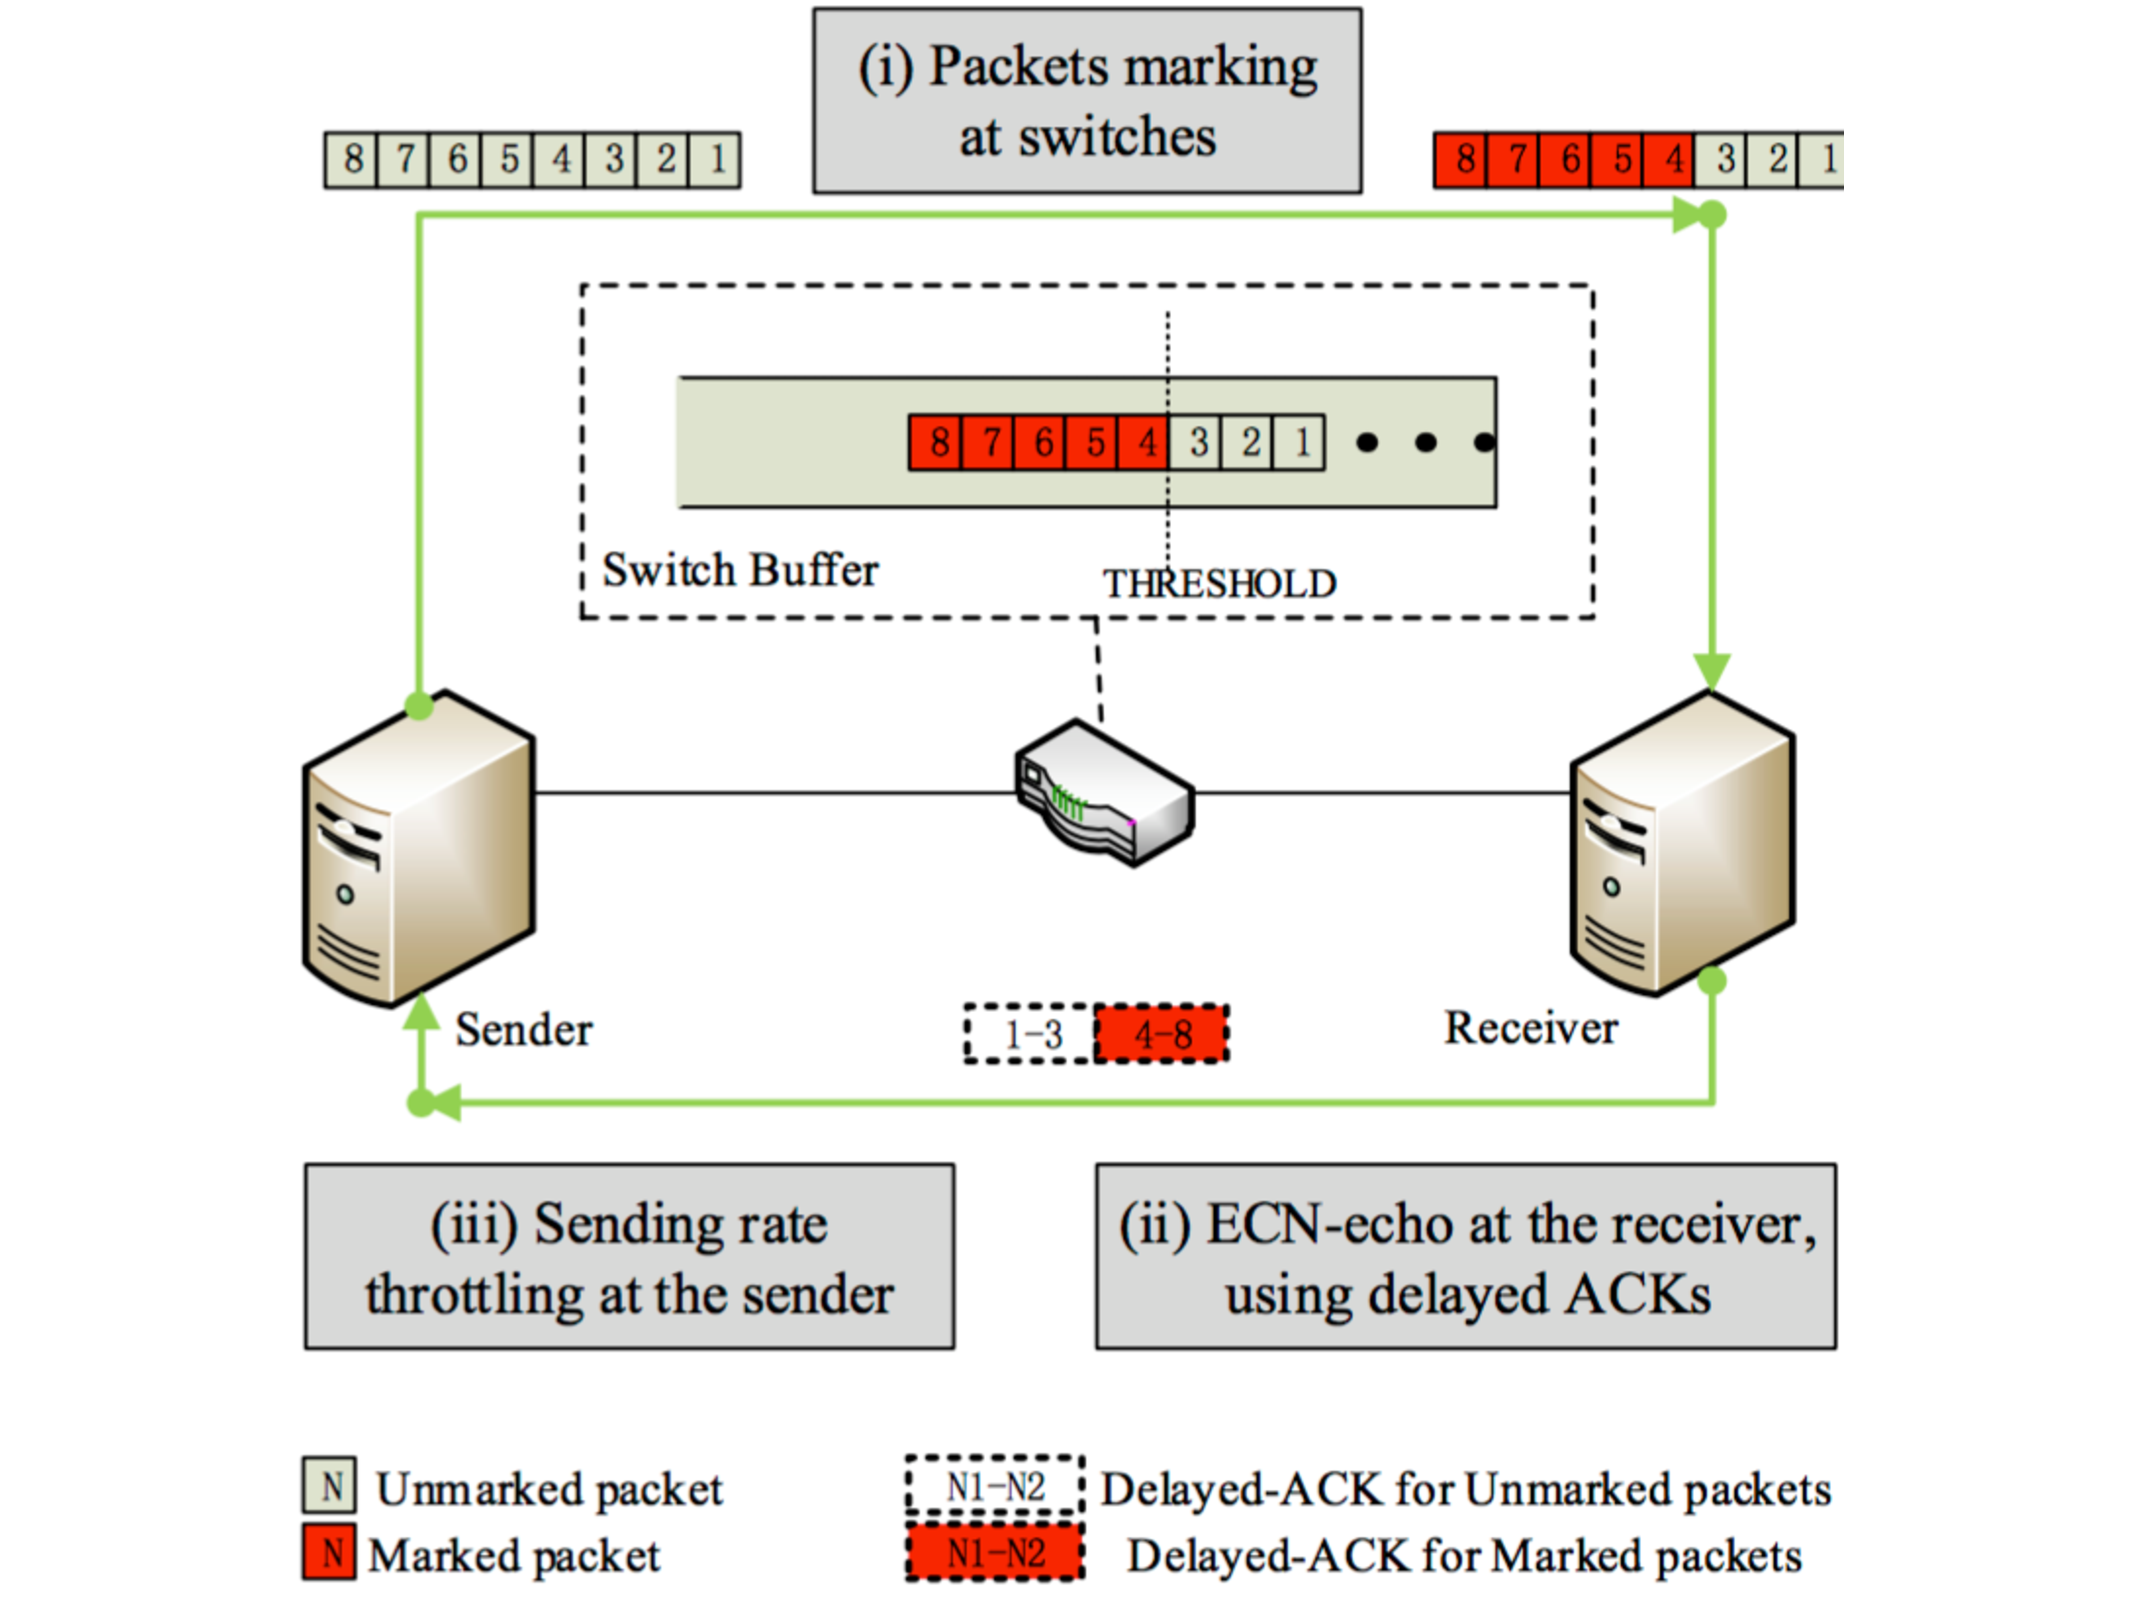
\includegraphics[width=0.9\columnwidth]{figures/others/model-process.pdf}
  \caption{基于ECN标记的数据中心速率控制过程,交换机上设置阈值,当排队队列超过阈值后,进行标记,发送端根据被标记的数据包比例,动态调整发送窗口}
  \label{model-process-fig}
\end{figure}

基于ECN标记的拥塞控制速率机制过程如图\ref{model-process-fig}所示:首先,发送端发送数据包给交换机,在交换机设置一个阈值,
当交换机队列长度超过阈值后,超过交换机设置队列设置阈值的数据包会被标记CE(和TCP不同,TCP会丢包)。
当接受端收到数据包后,检查数据包是否被标记CE,
如果发送的数据包被标记CE,那么给发送端回复的ACK中标记ECN。
发送端检查收到的ACK中被标记ECN的ACK的比例,以此来计算网络的拥塞程度$\alpha$,根据拥塞程度进行拥塞窗口的计算。

当网络中没有拥塞时(此RTT时间内没有被标记的数据包),滑动窗口每个RTT增加$(1-f_1(\alpha))$,
当网络中有拥塞时(此RTT时间内中有被标记的数据包),滑动窗口减小$f_2(\alpha)$倍。
其中$f_1(\alpha)$和$f_2(\alpha)$是关于拥塞程度$\alpha$的函数。
(\ref{Model-CA-eq})是基于ECN标记的拥塞避免阶段窗口变化的公式。

\begin{equation}
w=
\begin{cases}
w+(1-f_1(\alpha)) &\text{没有拥塞}\\
w \times (1-f_2(\alpha)) &\text{出现拥塞}
\end{cases}
\label{Model-CA-eq}
\end{equation}




\section{ECN标记流模型}\label{cha:model:introduction}




\begin{figure}[H] 
  \centering
  \includegraphics[width=0.9\columnwidth]{figures/others/senders.eps}
  \caption{N个发送端发送数据给1个接收端}
  \label{model-senders-fig}
\end{figure}

如图\ref{model-senders-fig}所示,假设N个发送端连接1个交换机,1个接收端连接在交换机上。
N个发送端使用公式(\ref{Model-CA-eq})进行拥塞控制窗口的计算。
交换机支持ECN标记,当交换机队列满足ECN标记条件时,发送到交换机的数据包会进行数据包标记。

\subsection{模型描述}

公式(\ref{fluid-model_window})$\sim$(\ref{fluid-model-q})是基于ECN标记的描述模型,
其中(\ref{fluid-model_window})表示的是窗口变化过程,其中,第一部分$\frac{1-f_1(\alpha)}{R(t)}$描述的是窗口增加的过程,
其中每个RTT窗口增加$1-f_1(\alpha)$。
$\frac{w_i(t)f_2(\alpha)}{R(t)}p(t-R^*)$描述的是窗口减小的过程,当发生拥塞时,窗口减小$\frac{w_i(t)f_2(\alpha)}{R(t)}$。
其中$p(t-R^*)$表示的是否出现ECN标记,当$p(t-R^*)=1$时,表示ACK中有ECN标记,当$p(t-R^*)=0$时,表示ACK中没有ECN标记,
此时网络中没有拥塞。

公式(\ref{fluid-model_queue})表示的是交换机队列变化,
$ \sum_{i=1}^N{\frac{w_i(t)}{R(t)}}$表示的是发送到交换机的数据包,
假设交换机的转发速率是C pkt/s,那么,交换机的队列长度是$\sum_{i=1}^N{\frac{w_i(t)}{R(t)}}-C \label{fluid-model_queue}$。

公式(\ref{fluid-model-q})是交换机是否进行标记,当交换机队列满足一定条件$F({q}(t))==1$时,
进行标记的函数$\widehat{p}(t)=1$,否则,$\widehat{p}(t)=0$。
 \begin{align}
&\frac{dw_i}{dt}=\frac{1-f_1(\alpha)}{R(t)}-\frac{w_i(t)f_2(\alpha)}{R(t)}p(t-R^*)  \label{fluid-model_window} \\
&\frac{dq}{dt}= \sum_{i=1}^N{\frac{w_i(t)}{R(t)}}-C \label{fluid-model_queue}  \\
&\widehat{p}(t)=1_{F({q}(t))==1}  \label{fluid-model-q}
\end{align}




\subsection{模型实例}

本章节,我们使用DCTCP\cite{DCTCP}来验证模型,DCTCP协议在交换机上设置阈值K,
当交换机的队列超过K时,数据包被打标记,同时在发送端滑动平均拥塞程度$\alpha$:

\begin{equation}
\alpha=(1-g)\times \alpha+g\times F
\label{Model-alpha-eq}
\end{equation}

其中,g为滑动平均因子,F为当前RTT中被标记ECN的数据包,
当前滑动平均拥塞程度$\alpha$为上一个RTT的打标记的ECN比例F和当前计算的平均拥塞程度的比例值。
在DCTCP中,$f_1(\alpha)=0$,$f_2(\alpha)=\frac{\alpha}{2}$,
将$f_1(\alpha)$和$f_2(\alpha)$带入(\ref{Model-CA-eq})得到拥塞控制函数:

\begin{equation}
w=
\begin{cases}
w+1 &\text{没有拥塞}\\
w \times (1-\frac{\alpha}{2}) &\text{出现拥塞}
\end{cases}
\label{Model-CA-DCTCP-eq}
\end{equation}
同时把$f_1(\alpha)$和$f_2(\alpha)$带入(\ref{fluid-model_window})$\sim$(\ref{fluid-model-q}),
并且改动(\ref{Model-alpha-eq}),得到:

 \begin{align}
&\frac{dw_i}{dt}=\frac{1}{R(t)}-\frac{w_i(t)\alpha}{2R(t)}p(t-R^*)  \label{DCTCP-fluid-model_window} \\
&\frac{dq}{dt}= \sum_{i=1}^N{\frac{w_i(t)}{R(t)}}-C \label{DCTCP-fluid-model_queue}  \\
&\frac{d\alpha_i}{dt}=\frac{g}{R(t)}(p(t-R^*)-\alpha_i(t)) \label{DCTCP-model_alpha} \\
&\widehat{p}(t)=1_{q(t))>K}  \label{DCTCP-fluid-model-q}
\end{align}

其中,(\ref{DCTCP-fluid-model_window})是描述的是DCTCP的窗口,
(\ref{DCTCP-fluid-model_queue})描述的是队列长度,当没有出现拥塞时,拥塞窗口每个RTT增加1,当出现拥塞时,滑动拥塞窗口减小$\frac{\alpha}{2}$。
特别的,(\ref{DCTCP-model_alpha})是描述的拥塞程度$\alpha$,
(\ref{DCTCP-fluid-model-q})中被标记的条件是队列长度大于K。
设置g=1/16,C=10Gbps,N=2,K=64,
图\ref{DCTCP-analysis-fig}是对DCTCP实例化的模型进行的验证并且使用ns-2和模型结果进行对比的结果。

\begin{figure}[h]
\centering
\subcaptionbox{$\alpha$}
 {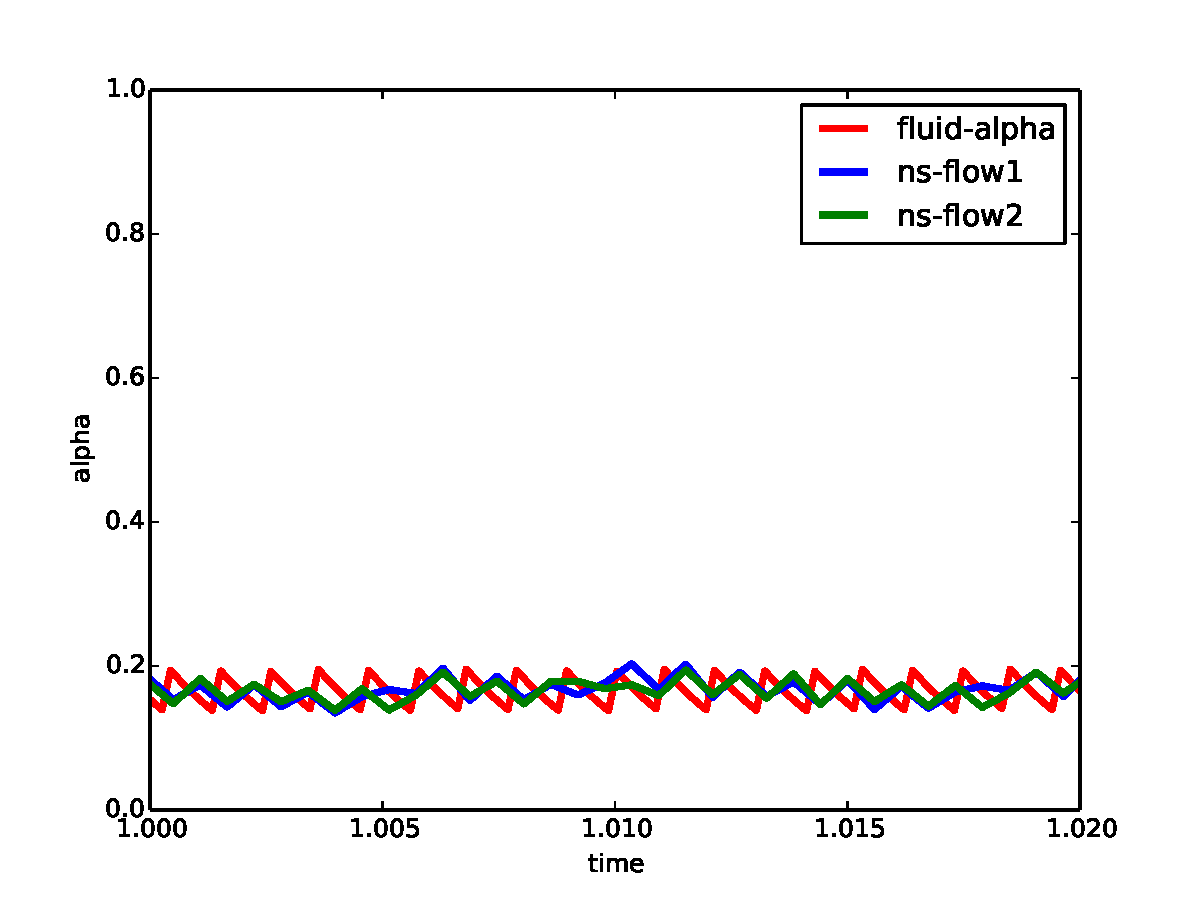
\includegraphics[width=0.32\columnwidth]{figures/others/DCTCP/alpha.pdf}}
\subcaptionbox{队列长度}
{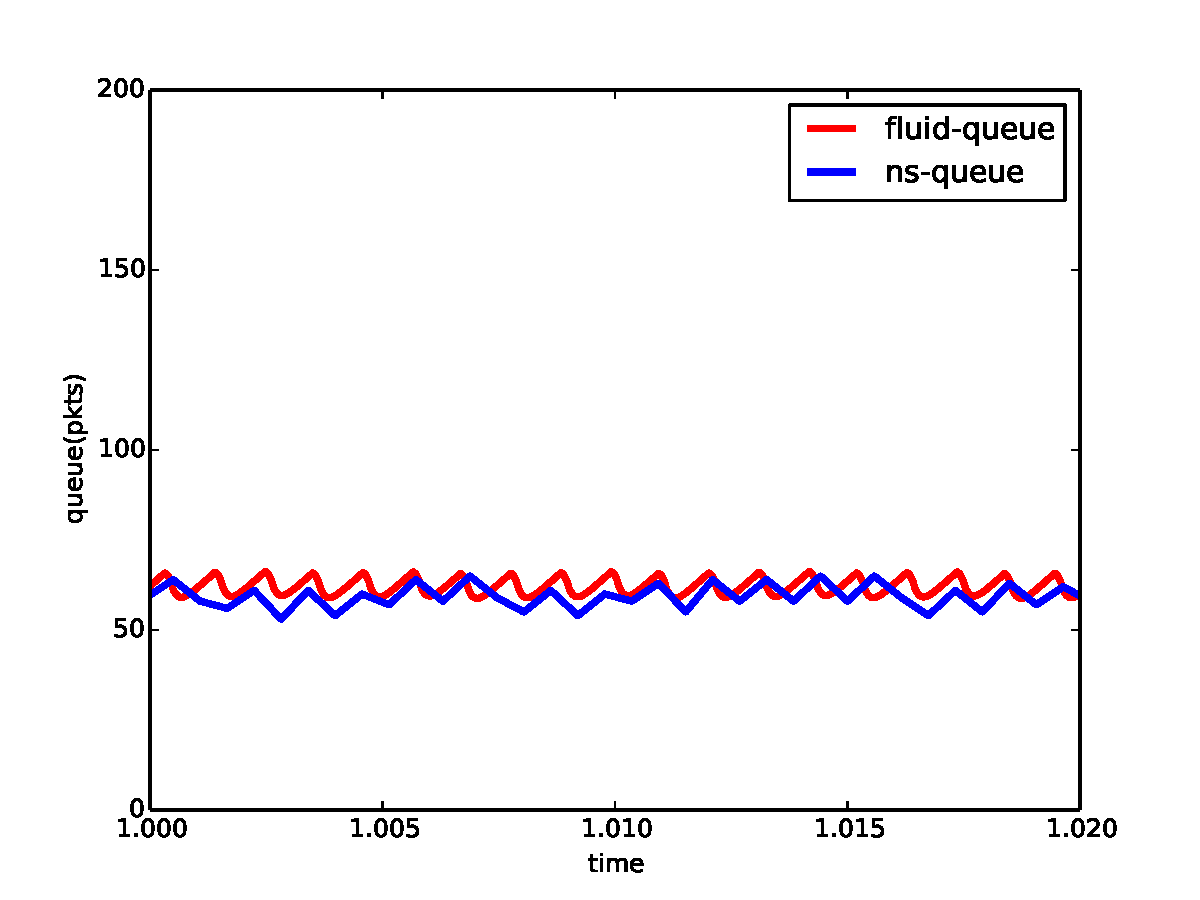
\includegraphics[width=0.32\columnwidth]{figures/others/DCTCP/queue.pdf}}
\subcaptionbox{窗口大小}
{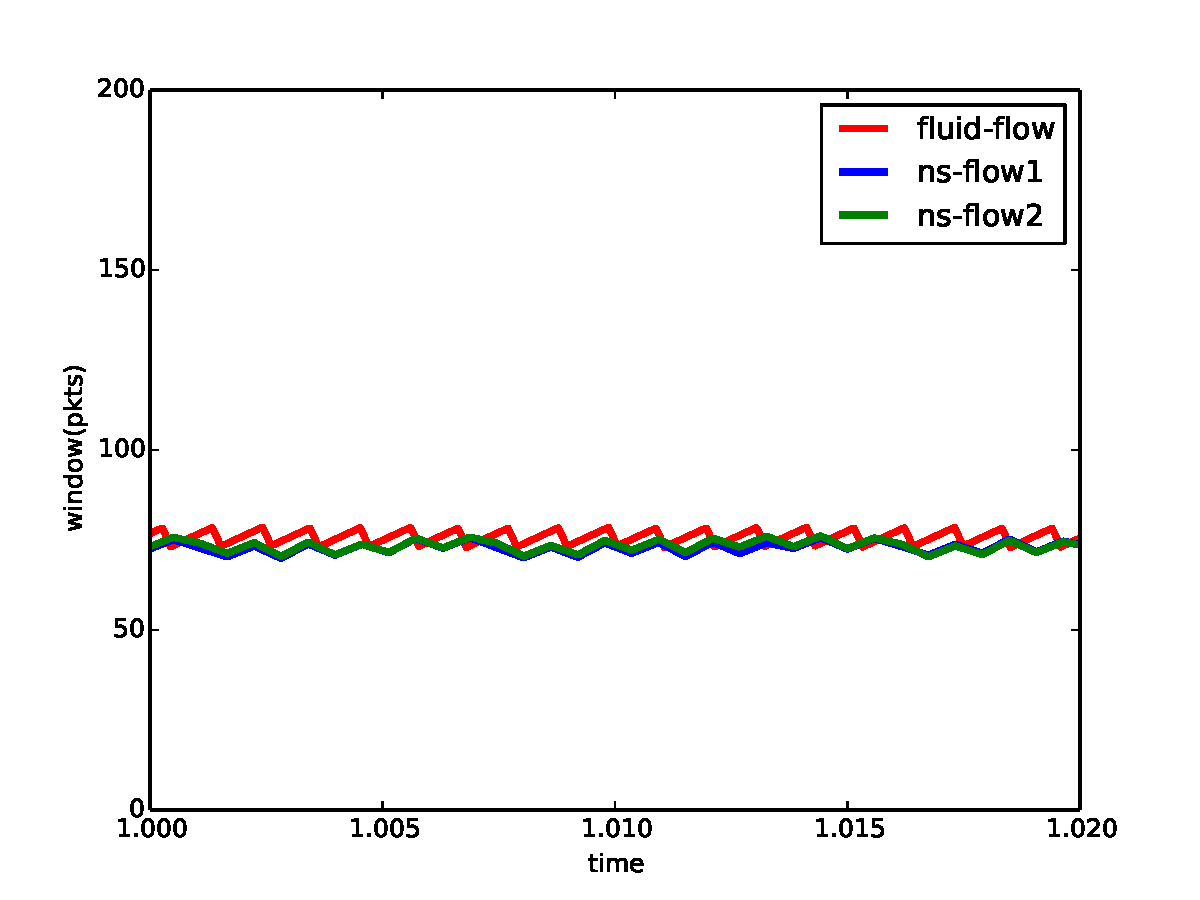
\includegraphics[width=0.32\columnwidth]{figures/others/DCTCP/window.pdf}}
\caption{DCTCP中标记ECN流模型推算结果和ns-2下结果对比}
\label{DCTCP-analysis-fig}
\end{figure}

图\ref{DCTCP-analysis-fig}(a)描述的是拥塞程度$\alpha$,
图\ref{DCTCP-analysis-fig}(b)描述的是队列长度,
图\ref{DCTCP-analysis-fig}(c)描述的是拥塞窗口,
我们可以发现,通过模型进行描述推倒的结果和仿真的结果基本相同。
因此,使用模型可以有效的描述基于ECN标记的传输协议。

\section{本章小结}
本章中,我们介绍了基于ECN标记的流模型。
我们介绍了基于ECN标记的流模型的场景和基于ECN标记的流模型。
最后,我们根据基于ECN标记的流模型实例化DCTCP,
得到DCTCP流模型,作为ECN标记的流模型的一个实例。